%-----------------------------------LICENSE------------------------------------%
%   This file is part of tikz_figures.                                         %
%                                                                              %
%   tikz_figures is free software: you can redistribute it and/or              %
%   modify it it under the terms of the GNU General Public License as          %
%   published by the Free Software Foundation, either version 3 of the         %
%   License, or (at your option) any later version.                            %
%                                                                              %
%   tikz_figures is distributed in the hope that it will be useful,            %
%   but WITHOUT ANY WARRANTY; without even the implied warranty of             %
%   MERCHANTABILITY or FITNESS FOR A PARTICULAR PURPOSE.  See the              %
%   GNU General Public License for more details.                               %
%                                                                              %
%   You should have received a copy of the GNU General Public License along    %
%   with tikz_figures.  If not, see <https://www.gnu.org/licenses/>.           %
%------------------------------------------------------------------------------%

% Use the standalone class for displaying the tikz image on a small PDF.
\documentclass[crop, tikz]{standalone}

% Import the tikz package to use for the drawing.
\usepackage{tikz}

% Needed for blackboard bold C.
\usepackage{amssymb}

% The arrow and decorations packages are used for the LaTeX arrow.
\usetikzlibrary{arrows.meta, decorations.markings}

% Begin the document.
\begin{document}

    % Draw the figure.
    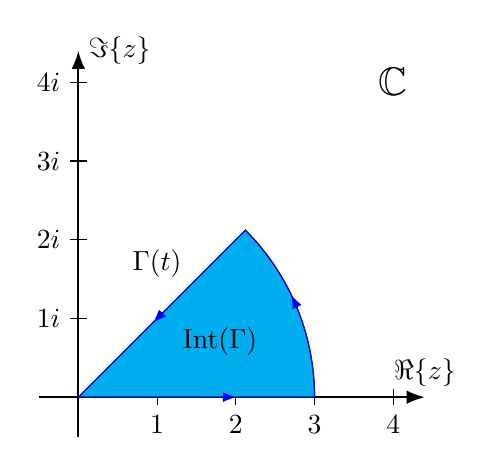
\begin{tikzpicture}[
        > = Latex,
        ->-/.style = {%
            decoration = {%
                markings,
                mark = at position 0.24 with \arrow{>},
                mark = at position 0.52 with \arrow{>},
                mark = at position 0.84 with \arrow{>}
            },
            postaction = {decorate}
        }
    ]

        % Coordinates for points on the curve.
        \coordinate (P1) at (0, 0);
        \coordinate (P2) at (3, 0);

        % Axes.
        \begin{scope}[thick]
            \draw[->] (-0.5, 0.0) to (4.4, 0.0) node[above] {$\Re\{z\}$};
            \draw[->] (0.0, -0.5) to (0.0, 4.4) node[right] {$\Im\{z\}$};
        \end{scope}

        % Axes Labels.
        \foreach\n in {1, 2, 3, 4}{%
            \draw (\n,3pt) to (\n,-3pt) node [below] {$\n$};
            \draw (3pt,\n) to (-3pt,\n) node [left]  {$\n{i}$};
        }

        % Draw the sector, shading the interior cyan.
        \draw[fill = cyan] (P1) to (P2) arc(0:45:3) to cycle;
        \draw[blue, ->-] (P1) to (P2) arc(0:45:3) to cycle;

        % Labels.
        \node at (4.0, 4.0) {\Large{$\mathbb{C}$}};
        \node at (1.0, 1.7) {\normalsize{$\Gamma(t)$}};
        \node at (1.8, 0.7) {\normalsize{$\textrm{Int}(\Gamma)$}};
    \end{tikzpicture}
\end{document}
